
\chapter{Planteamiento del proyecto}

En este cap\'\i tulo vamos a describir las ideas y contexto en el que vamos a desarrollar el contenido del proyecto.

\section{Descripci\'on}
Cuando un departamento de Recursos Humanos o una empresa de reclutamiento se enfrenta a una petici\'on para
cubrir un puesto vacante o de nueva creaci\'on, el proceso suele llevarse a cabo en diversas fases, que 
podr\'\i amos describir del siguiente modo \cite{proceso_seleccion1}:
\begin{enumerate}
\item {\bf Preselección}: etapa inicial en la que se detectan candidatos adecuados para el perfil buscado, bien recurriendo a 
anuncios en portales especializados, bien con b\'usquedas personalizadas de perfiles. En esta etapa se elabora una lista 
de candidatos que pasar\'an a las siguientes fases del proceso, descartando aquellos cuyas competencias no sean las adecuadas
para el puesto. 
\item {\bf Entrevista inicial}: en esta etapa los candidatos seleccionados en la etapa anterior son contactados para  
conseguir ampliar la informaci\'on de la que se dispone sobre ellos  (por ejemplo sobre las aptitudes
particulares y experiencias previas consignadas en el CV), y verificar el inter\'es y compromiso del candidato
con respecto a la oferta.
\item {\bf Informe}: tras la entrevista inicial, se seleccionan los mejores candidatos para el puesto, y se realiza un informe
donde se consignan los datos originales (el CV, por ejemplo) y los datos a\~nadidos en el curso de la entrevista inicial.
\item {\bf Presentaci\'on de candidatos}: el empleador recibe el informe elaborado en el punto anterior, y selecciona aquellos
que mejor se ajusten a sus necesidades, muy habitualmente realizando nuevas entrevistas con ellos.
\item {\bf Decisi\'on}: es el momento en que se elige el candidato al que se se le va a ofrecer el puesto, etapa en la 
que puede complementarse la informaci\'on recogida hasta el momento con referencias recabadas de anteriores empleadores.
\item {\bf Oferta}: etapa en la que la empresa presenta al candidato la oferta en firme, habitualmente por escrito, consignando 
la voluntad de la empresa de incorporar al candidato y los detalles econ\'omicos. 
\item: {\bf Seguimiento}:  para comprobar que una vez incorporado a la empresa, tanto empleado como empleador est\'an conformes con
el resultado del proceso.
\end{enumerate}

Tradicionalmente, el comienzo de este proceso, la detecci\'on de candidatos, se realizaba en numerosas ocasiones 
a trav\'es de anuncios en prensa,
bases de datos de candidatos construidas a lo largo del tiempo, y la explotaci\'on de la red de contactos personales del entorno 
del empleador. Hoy por hoy, estos m\'etodos tradicionales han sido complementados, y algunos dir\'\i an que pr\'acticamente
suplantados, por m\'etodos que explotan la informaci\'on contenida en la web. 

Los t\'ecnicos de selecci\'on se enfrentan a un mundo muy diverso donde tanto la difusi\'on de los 
posibles puestos como la informaci\'on sobre los candidatos para los mismos est\'a diseminada en numerosos
formatos, teniendo un papel preponderante diversas plataformas o portales web (InfoJobs, Monster, etc.)
y redes sociales en general (LinkedIn, Twitter, Facebook, Instagram, etc.). Desde el punto de vista del t\'ecnico de selecci\'on, las
primeras contienen mucha informaci\'on sobre las aptitudes de los posibles candidatos, sus conocimientos, formaci\'on y 
experiencia, ya que son portales donde los propios usuarios consignan sus curricula vitae, y tambi\'en sobre su situaci\'on laboral
actual y expectativas. En el segundo grupo de fuentes, las redes sociales, hay algunas que tienen el car\'acter espec\'\i fico 
de las primeras (LinkedIn es el ejemplo m\'as claro), y hay otras en las que se consigna informaci\'on diversa, llam\'emoslas de 
prop\'osito general, tal vez en mayor medida personal que profesional.

El objetivo de nuestro proyecto es complementar el 
trabajo habitual de un departamento de Recursos Humanos o de un seleccionador de personal en
los portales y redes sociales dedicados al mundo laboral, con informaci\'on laboral extra\'\i da 
de fuentes menos est\'andar, como son las redes sociales de prop\'osito general. 
Estas redes son a menudo aprovechadas por los usuarios para difundir mensajes relacionados con su actividad
laboral, y una descripción de su actividad en las redes es relevante desde el punto de vista 
de un reclutador, en la medida que da informaci\'on del compromiso de la persona con su actividad, su valoración por
parte de otros usuarios, su proactividad, etc.

En este trabajo hemos elegido la red social Twitter por diversos motivos: es una red muy dinámica, fácil de usar, rápida y divertida,
que involucra cientos de millones de usuarios activos en todo el mundo: 328 millones según la web de la red. El crecimiento del número 
de usuarios fue casi exponencial entre 2010 y 2014, si bien últimamente la velocidad a la que adquiere nuevos usuarios ha perido intensidad.
Es también una red que, desde sus orígenes, ha puesto a disposición de los interesados los mecanismos necesarios para acceder a 
la información que atesora, con ciertas limitaciones, pero de forma relativamente sencilla. 



\myfigure{
\begin{tabular}{cc}
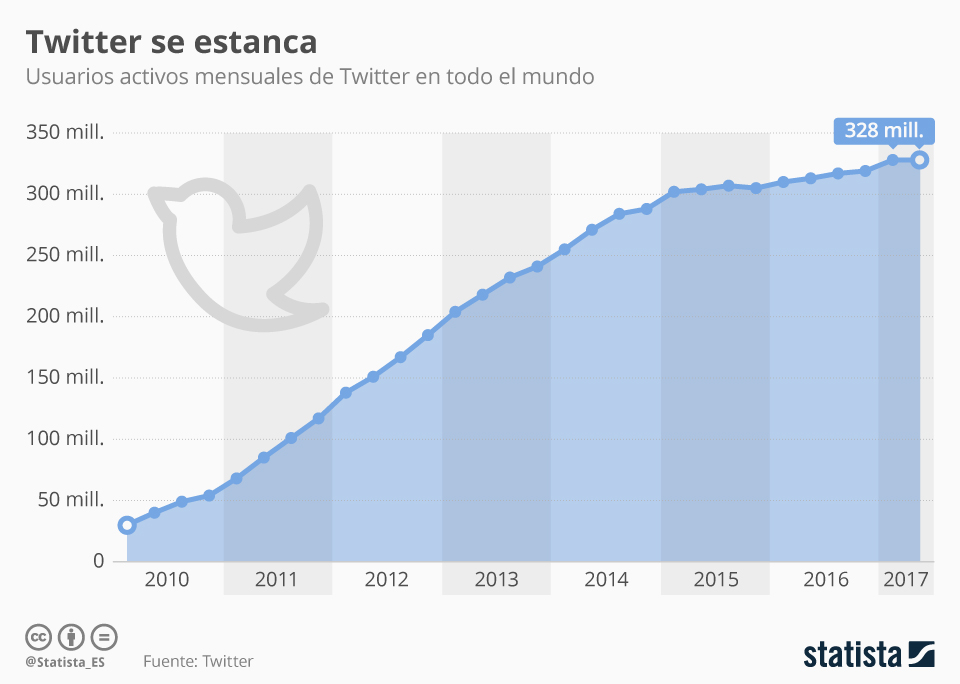
\includegraphics[width=0.4\textwidth]{usuarios_de_twitter}
&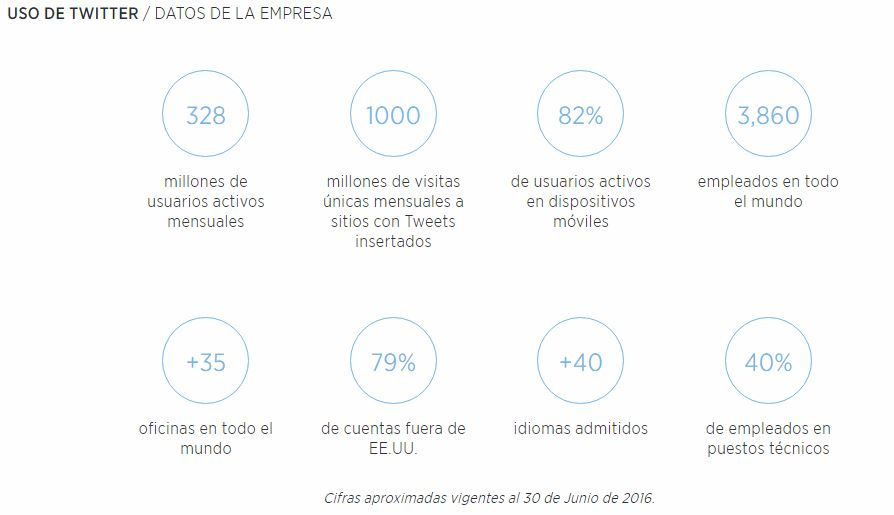
\includegraphics[width=0.4\textwidth]{twitter_uso_y_empresa}
\end{tabular}
\figcaption{Twitter: evolución del número de usuarios (Statista 2017, 
            \url{https://es.statista.com/grafico/10476/el-numero-de-usuarios-de-twitter-se-estanca })
			y datos de la empresa, \url{https://about.twitter.com/es/company }.}
\label{fig:Twitter_uso} }


Esta red da cabida a relaciones diversas, entre usuarios de variada índole. Dado que muchos de los usuarios 
publican información relacionada con su ocupación laboral, es natural esperar que en Twitter 
se formen comunidades de individuos que comparten interés en diferentes aspectos de dicho ámbito.
Nuestro propósito es definir e implementar un proceso que permita agregar información referente a 
esas comunidades a un determinado proceso de selección.

Observemos las dos siguientes ofertas de trabajo aparecidas recientemente (Septiembre 2017) en LinkedIn,
incluyendo los requisitos solicitados a los posibles candidatos:

\myfigure{\begin{tabular}{cc}
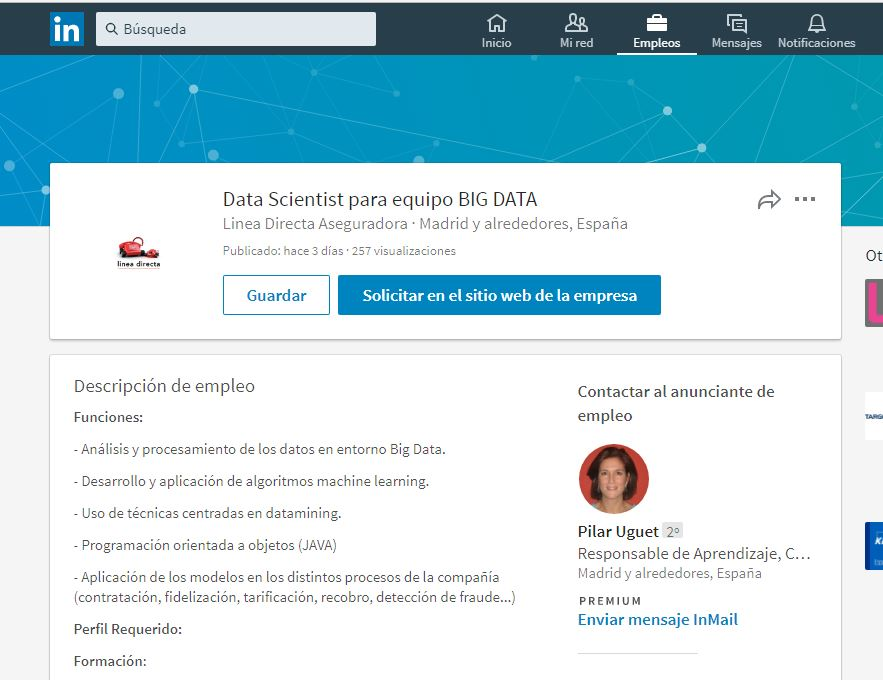
\includegraphics[width=0.4\textwidth]{oferta1_1}
&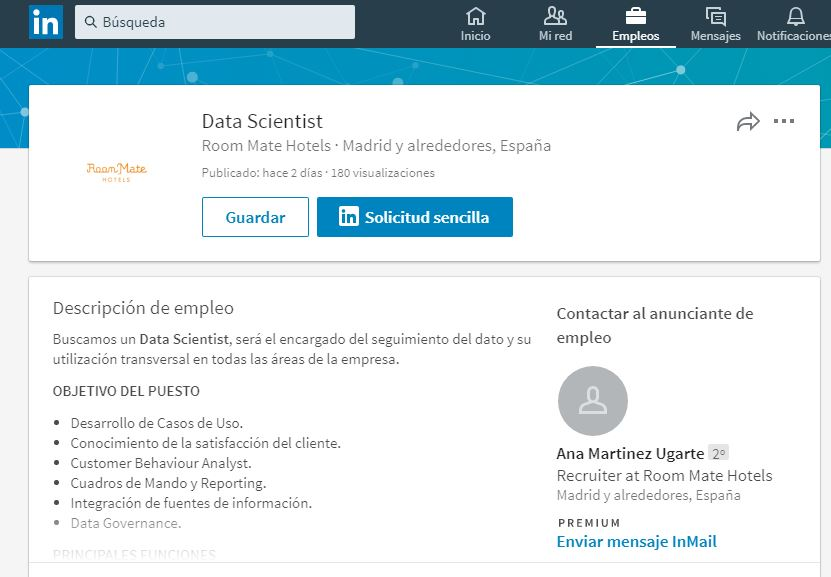
\includegraphics[width=0.4\textwidth]{oferta2_1}
\end{tabular}
\figcaption{Dos ofertas de empleo.}
\label{fig:ofertas_descripcion} }


\myfigure{\begin{tabular}{cc}
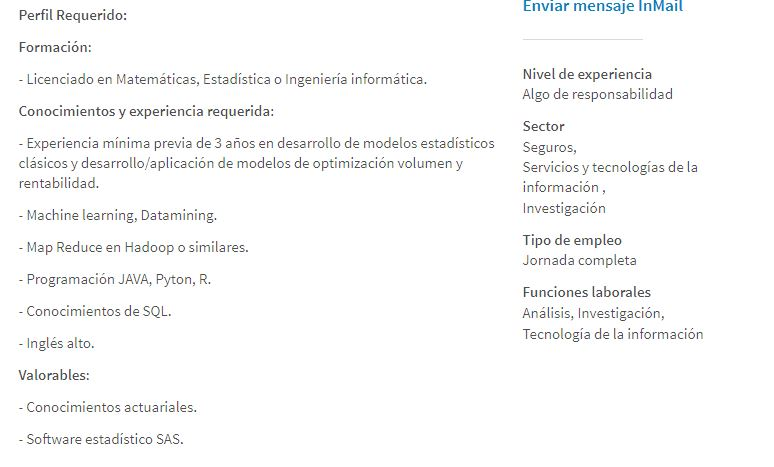
\includegraphics[width=0.4\textwidth]{oferta1_2}
&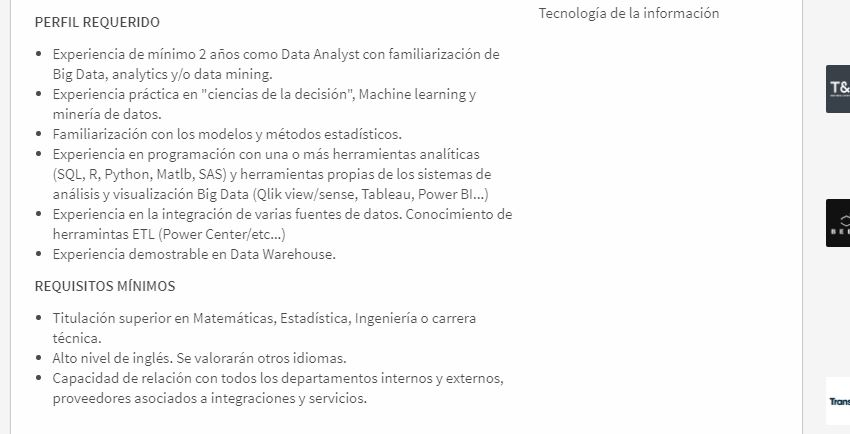
\includegraphics[width=0.4\textwidth]{oferta2_2}
\end{tabular}
\figcaption{Requisitos de las dos ofertas de empleo.}
\label{fig:ofertas_requisitos} }

En ambos casos, entre los requisitos se encuentran conocimientos sobre Python, R,
SQL, machine learning y data mining. Un reclutador probablemente usará esas palabras clave para buscar
los perfiles adecuados para alguno de los dos puestos, y construirá un conjunto de posibles candidatos (el
primer paso en nuestra descripción del proceso de contratación). En esta fase, y gracias a Octopus Data Insights,
nuestro reclutador contará con una ayuda extra. Octopus Data Insights le proporcionará una lista de usuarios
de Twitter que hayan publicado contenido en el que aparezcan esas palabras clave, que complementarán
el resultado que el reclutador haya obtenido por sus propios medios. La información proporcionada
por Octopus Data Insights resultará relevante también más adelante en el proceso,
cuando haya que tomar una decisión entre varios candidatos para determinar cuáles son los más adecuados para el 
puesto: usando la información de Twitter, los usuarios de la lista estarán ordenados según 
diversos criterios de relevancia.

El proceso para producir la información que ayudará al reclutador en el proceso es el siguiente:
\begin{enumerate}
\item Identificar los vocablos que determinan las habilidades que ha de poseer cualquier candidato
para la oferta en cuestión y extraer de Twitter aquellos tuits con contenido relacionado con ellos.
\item Dados esos tuits, construir un conjunto de usuarios, que entendemos como posibles candidatos 
a la oferta.
\item Usar la información publicada por los usuarios para determinar el grado de adecuación a la oferta
(serán más adecuados aquellos que hayan publicado información sobre todos los conocimientos requeridos que 
aquellos que solo hayan publicado sobre alguno de ellos, y más relevantes aquellos más activos, según el
número de tuits publicados sobre cada área).
\item Estudiar la relación entre los usuarios de este conjunto, y determinar los más relevantes en sentido
relativo (en términos de actividad en la red, cuáles son los más ``retuiteados", cuáles los más seguidos, etc.).
\end{enumerate}



\section{Contexto de negocio}
Lo que hay hecho y lo que no.
\section{Objetivos}
Lo que queremos conseguir, qué significa que lo hayamos conseguido.
\section{Hip\'otesis y limitaciones}
Aquí todo lo que asumamos al plantear el proyecto, y hasta dónde puede llegar. Límites del uso de la información
de las redes sociales, límites del proceso en sí (ventana temporal, no detección de todos los candidatos, etc.).

La hipótesis fundamental que estamos haciendo al iniciar este proceso, es que la actividad en Twitter
acerca de un determinado tema (por ejemplo, publicar algo relacionado con Python), supone
que el usuario en cuestión tiene conocimientos sobre dicho tema (en nuestro caso, entenderíamos que ese
usuario posee conocimientos de Python). Esto es cuestionable, por supuesto, pero también ponderable
si tenemos en cuenta que la actividad no sea esporádica. Si un usuario publica sobre un tema
en numerosas ocasiones, la hipótesis de que ese tema no le resulta ajeno, va cobrando fuerza.

Entre las limitaciones de las que adolece el proceso definido para llevar a cabo el proyecto, se encuentran las 
siguientes:
\begin{enumerate}
\item En general, no todos los posibles candidatos tienen por qué usar Twitter, y por tanto habrá muchos que 
queden directamente fuera de nuestro proceso.
\item Los tuits utilizados en el proceso están sujetos a una ventana temporal. Habrá muchos candidatos,
usuarios de Twitter, que no aparezcan en nuestros registros, por no presentar actividad durante ese tiempo.
\item Twitter impone limitaciones en la cantidad de información a la que deja acceder, y por ello, también es
posible que los usuarios pierdad visibilidad en este proceso, 
porque el contenido publicado por ellos no se encuentre entre el proporcionado por la red social durante el proceso
de extracción de datos.
\end{enumerate}


Otra limitación del proceso es que la información que obtenemos de la red es a nivel de usuario de Twitter. 
La dirección de correo o el nombre verdadero de la persona en cuestión, o cualquier dato que pudiera identificarla
no está necesariamente disponible en la aplicación, salvo que el usuario lo haya querido hacer público explícitamente. 
Esta información, y la forma en que se utilice, es clave para la usabilidad del resultado del proyecto, en dos aspectos principales:
\begin{enumerate}
\item para que el reclutador pueda hacer uso de la información, la persona ha de estar identificada, lo suficientemente
como para abrir un canal de comunicación entre el reclutador y el posible candidato.
\item desde el punto de vista de la comercialización del resultado del proyecto, el hecho de identificar usuarios en una red
social y usar esa información con fines lucrativos, ha de ser implementado de forma muy cuidadosa. El impacto de la Ley 
Orgánica de Protección de Datos de Carácter Personal (LOPD) es muy relevante en nuestro proyecto, y merece un apartado especial.
Nos ocupamos de ello en la sección \ref{subsection:LOPD}.
\end{enumerate}
En relación al primer punto, evidentemente proporcionar un usuario de Twitter ya es abrir un canal de
comunicación. Sin embargo, solo la información de las publicaciones del usuario no es suficiente para 
incluirlo en un proceso de selección, incluso antes del primer contacto entre reclutador y candidato,
y el primero probablemente  necesitará más información (por ejemplo un CV) para considerar al segundo. 
Una forma de solventarlo sería cruzar la información de Twitter (el nombre de usuario)
con la contenida en otros portales (como LinkedIn,  Facebook, Academia.edu, ResearchGate, Glassdoor, etc.),
ya que a menudo el usuario de Twitter es parte de los datos consignados en los CV. Esta extensión
del proyecto la hemos dejado deliberadamente fuera del planteamiento de este proyecto, aunque sería 
{\em conditio sine qua non} para una implementación comercializable del proyecto.




\subsection{La Ley Orgánica 15/1999, de 13 de diciembre, de Protección de Datos
de Carácter Personal}
\label{subsection:LOPD}


\myfigure{

\includegraphics[width=0.4\textwidth]{LOPD1}
\figcaption{Ayuda Ley de Protección de Datos
           \url{https://ayudaleyprotecciondatos.es/2010/09/16/redes-sociales-empresas-y-proteccion-de-datos/ }}
\label{fig:LOPD1} }



Otra forma, sería implementar un sistema que 
cuando un usuario de Twitter fuera a ser incluido en uno de los procesos 
